\chapter{ATIVIDADES DESENVOLVIDAS}

Neste capítulo falaremos sobre as atividades que foram desenvolvidas ao longo do projeto integrador, discutindo as principais ações que tomamos para o desenvolvimento do sistema de locação de imóveis. As próximas seções demonstrarão aspectos do desenvolvimento do website.



%Adicione aqui um parágrafo introdutório para que o capítulo não comece ``vazio'' e a leitura não entre diretamente na primeira seção. Você pode começar o parágrafo falando do assunto e dando continuidade nas seções seguintes ou começar com um parágrafo genérico que descreve o que os leitores encontrarão. Exemplo:

%\textit{``Esse capítulo apresentará...''}





\section{ESCOPO DO PROJETO}
Após reuniões iniciais, definimos que o escopo do projeto será estruturado da seguinte forma:


%O escopo deste projeto define os limites e as funcionalidades do sistema de locação de imóveis que será desenvolvido. É essencial esclarecer o que está incluído e o que está excluído do projeto para evitar mal-entendidos futuros.

\begin{itemize}
    \item \textbf{Inclusões:}
    \begin{itemize}
        \item Cadastro de imóveis disponíveis para locação;
        \item Agendamento de visitas para os locatários;
        \item Busca e filtragem de imóveis com base em critérios como localização, tipo de imóvel e preço;
        \item Interface para que locadores gerenciem suas propriedades;
        \item Sistema de chats para comunicação entre locadores e locatários;
        \item Modelo de contrato de locação, acessível aos usuários, para que possam compreender os principais aspectos legais desse tipo de acordo.
    \end{itemize}
    
    \item \textbf{Exclusões:}
    \begin{itemize}
        \item Gestão de pagamentos e contratos de locação.
        \item Serviços adicionais como manutenção e suporte pós-locação.
    \end{itemize}
\end{itemize}

\subsection{Funcionalidades do Sistema}
As principais funcionalidades do sistema incluem:

\begin{itemize}
    \item \textbf{Cadastro de Usuários:}
    \begin{itemize}
        \item Permitir que locadores e locatários criem contas e façam login no sistema.
    \end{itemize}
    
    \item \textbf{Busca de Imóveis:}
    \begin{itemize}
        \item Permitir que os usuários busquem imóveis por diversos critérios, como localização, preço e tipo de imóvel.
    \end{itemize}
    
    \item \textbf{Cadastro de Imóveis:}
    \begin{itemize}
        \item Permitir que locadores cadastrem seus imóveis com informações detalhadas, incluindo fotos e descrições.
    \end{itemize}
    
    \item \textbf{Agendamento de Visitas:}
    \begin{itemize}
        \item Permitir que os locatários agendem visitas aos imóveis.
    \end{itemize}
    
    \item \textbf{Sistema de Chats:}
    \begin{itemize}
        \item Permitir comunicação em tempo real entre locadores e locatários para esclarecer dúvidas e discutir detalhes dos imóveis.
    \end{itemize}

    \item \textbf{Modelo de Contrato de Locação:}
    \begin{itemize}
        \item Disponibilizar um modelo de contrato de locação acessível aos usuários, proporcionando informações essenciais sobre os direitos e deveres de ambas as partes.
    \end{itemize}
\end{itemize}

\subsection{Levantamento de Requisitos}
\begin{table}[h!]
\centering
\caption{Requisitos Funcionais do Sistema}
\begin{tabular}{|c|p{10cm}|}
\hline
\textbf{Código do Requisito} & \textbf{Descrição do Requisito} \\
\hline
RF01 & O sistema deve permitir o cadastro de usuários. \\
\hline
RF02 & O sistema deve permitir a atualização dos dados do usuário, incluindo nome, e-mail, senha, telefones e foto de perfil. \\
\hline
RF03 & O sistema deve permitir ao usuário deletar sua conta. \\
\hline
RF04 & O usuário receberá um e-mail para verificar o endereço de e-mail informado. \\
\hline
RF05 & O usuário deve ser capaz de recuperar a sua senha caso a esqueça. \\
\hline
RF06 & O sistema deve permitir o cadastro de imóveis pelos locadores. \\
\hline
RF07 & O sistema deve permitir o envio de fotos e vídeos ao realizar o cadastro do imóvel. \\
\hline
RF08 & O sistema deve permitir a atualização dos dados dos imóveis, incluindo informações gerais, fotos e vídeos. \\
\hline
RF09 & O sistema deve possibilitar a busca de imóveis. \\
\hline
RF10 & O sistema deve permitir agendamentos de visitas. \\
\hline
RF11 & O sistema deve permitir ao usuário atualizar a data e a hora das visitas. \\
\hline
RF12 & O sistema deve permitir ao usuário cancelar visitas. \\
\hline
RF13 & O sistema deve ter um sistema de confirmação de visitas, garantindo que ambas as partes estarão disponíveis na hora marcada. \\
\hline
RF14 & O sistema deve incluir um sistema de chats para comunicação entre locadores e locatários. \\
\hline
RF15 & O sistema deve disponibilizar um modelo de contrato de locação para os usuários. \\
\hline
\end{tabular}
\label{tab:requisitos_funcionais}
\end{table}
\subsubsection{Requisitos Funcionais (RF)}
Os requisitos funcionais do sistema incluem:
\newpage




\subsubsection{Requisitos Não-Funcionais (RNF)}
Os requisitos não-funcionais incluem:

\begin{table}[h]
\centering
\caption{Requisitos Não Funcionais}
\begin{tabular} {|p{3cm}|p{10cm}|} 
\hline
\textbf{Identificador} & \textbf{Requisito} \\ \hline
RNF01 & O sistema deve ser acessível via dispositivos móveis. \\ \hline
RNF02 & O tempo de resposta para busca de imóveis deve ser inferior a 4 segundos. \\ \hline
RNF03 & O sistema deve garantir a segurança dos dados dos usuários. \\ \hline
RNF04 & O sistema deve ser compatível com os principais navegadores (Chrome, Firefox, Safari e Edge). \\ \hline
RNF05 & O sistema deve fornecer um tempo de carregamento de página inferior a 3 segundos. \\ \hline
RNF06 & O sistema deve ser escalável para acomodar o aumento no número de usuários e imóveis. \\ \hline
RNF07 & O sistema deve ser de fácil manutenção e atualização. \\ \hline
RNF08 & O sistema deve apresentar uma interface amigável e intuitiva, facilitando a navegação para todos os usuários. \\ \hline
\end{tabular}
\end{table}


\newpage
\section{BANCO DE DADOS}

A equipe optou pela utilização de um banco de dados relacional e que já tinhamos um certo grau de conhecimento o \textbf{MySQL}.
No sistema criado os dados são salvos, apagados, atualizados e coletados através de Models que realizam a conexão com o banco de dados.

\subsection{Diagrama Entidade-Relacionamento}

Na figura 1 esta apresentado o diagrama entidade-relacionamento criado durante o projeto.
\newpage
\begin{figure}[h!] 
    \centering
    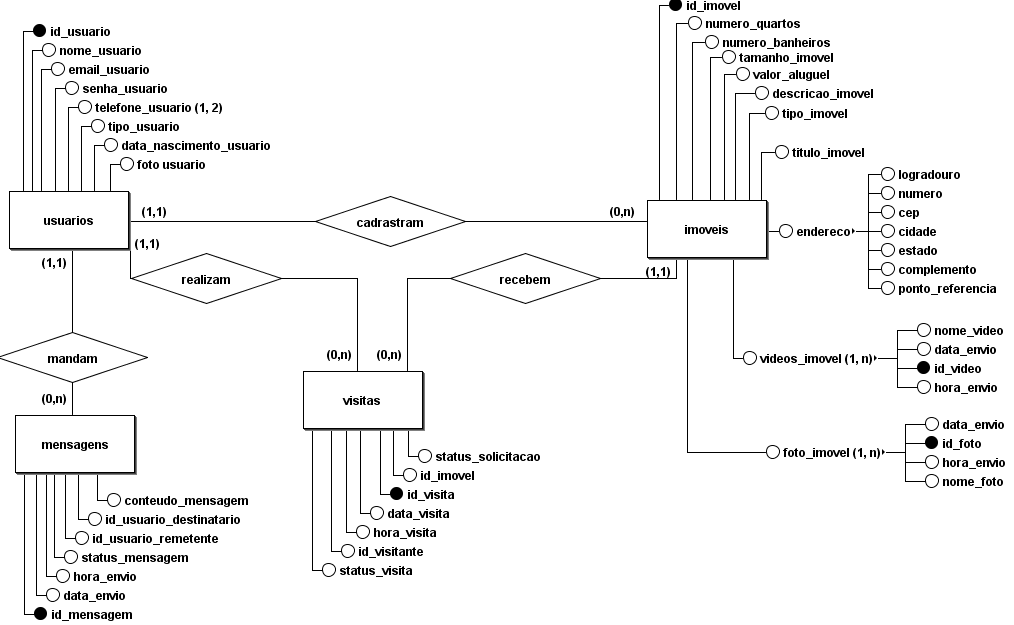
\includegraphics[width=\textwidth]{./img/Conceitual.png}
    
    \caption{Foto do Diagrama Entidade-Relacionamento (DER)}
    \label{fig:exemplo-imagem}
\end{figure}

\subsubsection{Entidades}
Agora vamos falar sobre as entidades e os atributos mostrados no diagrama\\


\setlength{\extrarowheight}{5pt} 

\begin{table}[htbp]
    \centering
    \caption{Usuários}
    \begin{tabular}{|p{5cm}|p{10cm}|} 
        \hline
        \textbf{Atributo} & \textbf{Função} \\
        \hline
        id\_usuario & Armazena o uuid completo do usuário \\ 
        \hline
        nome\_usuario & Armazena o nome completo do usuário \\ 
        \hline
        email\_usuario & Armazena o email do usuário para login e contato \\ 
        \hline
        senha\_usuario & Armazena a senha criptografada do usuário \\ 
        \hline
        telefone\_usuario(1,2) & Armazena até dois números de telefone do usuário \\ 
        \hline
        tipo\_usuario & Indica o tipo de usuario, podendo ser "PADRÃO", "PROPRIETÁRIO" e "ADMINISTRADOR" \\ 
        \hline
        data\_nascimento\_usuario & Armazena a data de nascimento do usuario \\ 
        \hline
    \end{tabular}
    \label{tab:usuarios}
\end{table}
\newpage
\begin{table}[htbp]
    \centering
    \caption{Imóveis}
    \begin{tabular}{|p{5cm}|p{10cm}|} 
        \hline
        \textbf{Atributo} & \textbf{Função} \\
        \hline
        id\_imovel & Armazena o uuid completo do imóvel \\ 
        \hline
        numero\_quartos & Armazena a quantidade de quartos do imóvel \\ 
        \hline
        numero\_banheiros & Armazena a quantidade de banheiros do imóvel \\ 
        \hline
        tamanho\_imovel & Armazena o tamanho em m\^2 do imóvel \\ 
        \hline
        valor\_imóvel & Armazena o valor em reais do imóvel \\ 
        \hline
        descricao\_imovel & Armazena a descrição do proprietário sobre o imóvel \\ 
        \hline
        tipo\_imovel & Armazena o tipo do imovel \\ 
        \hline
        titulo\_imovel & Armazena o título do imóvel \\ 
        \hline
        videos\_imovel & Armazena o tipo de imovel \\ 
        \hline
        endereco & Atributo composto que guarda as informações sobre o endereço do imóvel \\ 
        \hline
        videos\_imovel & Atributo composto e multivalorado que guarda as informações sobre os vídeos do imóvel \\ 
        \hline
        fotos\_imovel & Atributo composto e multivalorado que guarda as informações sobre as fotos do imóvel \\ 
        \hline
    \end{tabular}
    \label{tab:usuarios}
\end{table}


\begin{table}[htbp]
    \centering
    \caption{Visitas}
    \begin{tabular}{|p{5cm}|p{10cm}|} 
        \hline
        \textbf{Atributo} & \textbf{Função} \\
        \hline
        id\_visita & Armazena o uuid completo da visita \\ 
        \hline
        data\_visita & Armazena a data da visita \\ 
        \hline
        hora\_visita & Armazena a hora da visita \\ 
        \hline status\_solicitacao & Armazena o status da solicitacao da visita, "CONFIRMADA", "AGUARDANDO CONFIRMACAO" \\ 
        \hline status\_vista & Armazena status da visita, "REALIZADA", "NÃO REALIZADA" \\ 
        \hline
        id\_visitante  & Armazena o uuid do usuario que realizou a visita \\ 
        \hline
        
    \end{tabular} 
    \label{tab:usuarios}
\end{table}

\newpage
\begin{table}[htbp]
    \centering
    \caption{Mensagens}
    \begin{tabular}{|p{5cm}|p{10cm}|} 
        \hline
        \textbf{Atributo} & \textbf{Função} \\
        \hline
        id\_mensagem & Armazena o uuid completo da mensagem \\ 
        \hline
        data\_envio & Armazena a data de envio da mensagem \\ 
        \hline
        hora\_envio & Armazena a hora de envio da mensagem \\ 
        \hline
        status\_mensagem & Armazena o status da mensagem, "ENVIADA", "RECEBIDA" \\ 
        \hline
        id\_usuario\_remetente & Armazena o uuid de quem enviou a mensagem \\ 
        \hline
        id\_usuario\_destinatário & Armazena o uuid de quem recebeu a mensagem \\
        \hline
        conteudo\_mensagem & Armazena o conteudo da mensagem \\ 
        \hline
        
    \end{tabular}
    \label{tab:usuarios}
\end{table}

\subsubsection{Relacionamentos}

Agora vamos falar sobre os relacionamentos que cada entidade possui.

\begin{itemize}
    \item Usuarios - Cadastram - Imóveis: É um relacionamento (1:n), pois cada usuario poderá cadastrar "n" casas e cada casa é cadastrada por um
    único usuario.
    \item Usuarios - Mandam - Mensagens: É um relacionamento (1:n), pois cada usuario mandará "n" mensagens e cada mensagem é mandada por um único usuario
    \item Usuarios - Realizam - Visitas: É um relacionamento (1:n), pois cada usuario pode visitar "n" imóveis e cada visita é realizada por um único usuario
    \item Imoveis - Recebem - Visitas: É um relacionamento (1:n), pois cada imovel pode receber  "n" visitas e cada visita é realizada em um único imovel

\end{itemize}

\subsection{Modelo Entidade-Relacionamento}

Iremos agora mostrar a modelagem entidade-relacionamento criada durante o projeto.

\newpage
\begin{figure}[h!] 
    \centering
      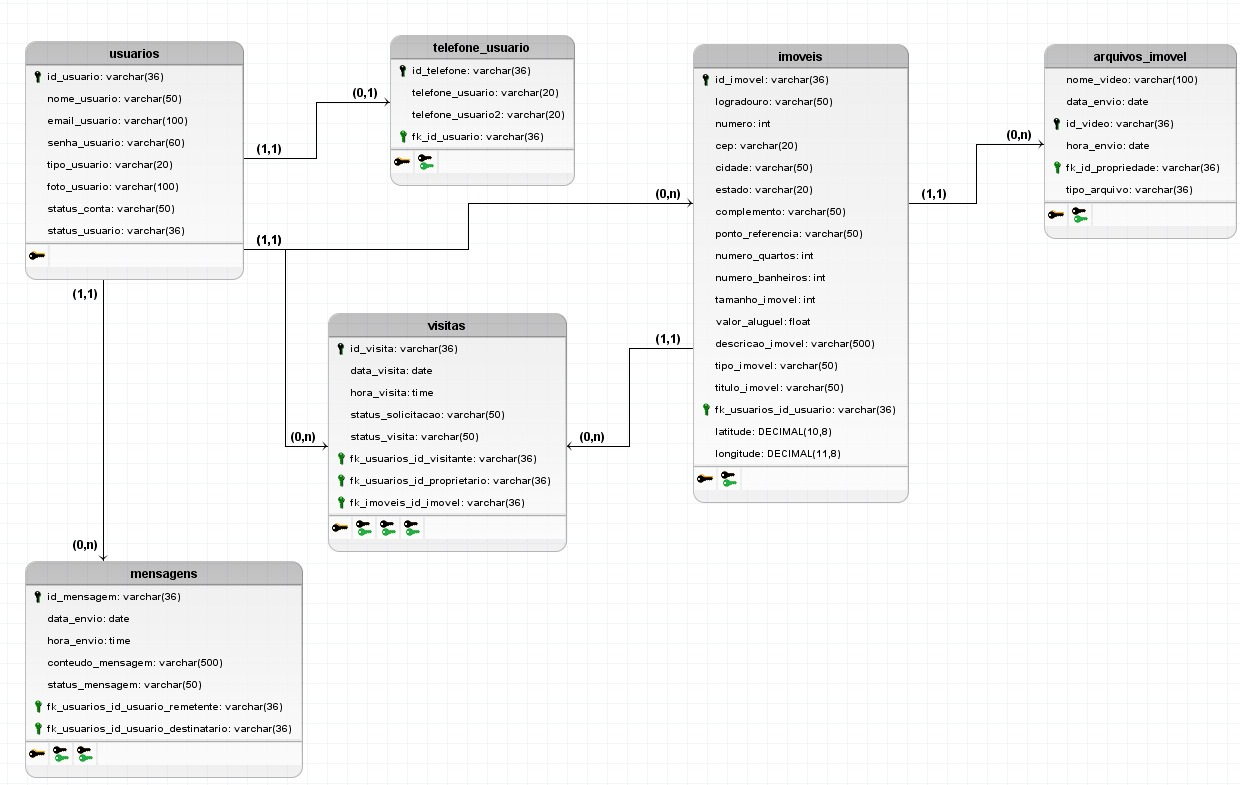
\includegraphics[width=\textwidth]{./img/Logico.jpeg}
    \caption{Foto do Diagrama Entidade-Relacionamento (DER)}
    \label{fig:exemplo-imagem}
\end{figure}


\subsubsection{Tipos de dados}

Os tipos de dados que cada atributo recebeu foram escolhidos para garantir a quantidade adequada de armazenamento e integridade dos dados. Mas existem dois que são especias para aquela função.

\begin{itemize} 
    \item \textbf{VARCHAR(36)}: Este tipo é utilizado para armazenar o UUID (Identificador Único Universal) gerado pelo sistema. O tamanho de 36 caracteres foi escolhido por conta do UUID gerado possuir exatamente 36 caracteres.
    \item \textbf{VARCHAR(60)}: Este tipo é destinado ao armazenamento da senha do usuário. A senha digitada pelo usuário será criptografada, resultando em um tamanho de até 60 caracteres. 


\end{itemize}


\subsubsection{Chaves Estrangeiras}

\begin{table}[htbp]
    \centering
    \caption{Imóveis}
    \begin{tabular}{|p{8cm}|p{7cm}|} 
        \hline
        Chave & Origem\\
        \hline
        fk\_usuarios\_id\_usuario & Tabela: Usuarios\\
        \hline
    \end{tabular}
    \label{tab:Imoveis}
\end{table}

\begin{table}[htbp]
    \centering
    \caption{videos\_imovel}
    \begin{tabular}{|p{8cm}|p{7cm}|} 
        \hline
        Chave & Origem\\
        \hline
        fk\_id\_propriedade & Tabela: Imoveis\\
        \hline
    \end{tabular}
    \label{tab:Imoveis}
\end{table}

\begin{table}[htbp]
    \centering
    \caption{fotos\_imovel}
    \begin{tabular}{|p{8cm}|p{7cm}|} 
        \hline
        Chave & Origem\\
        \hline
        fk\_id\_propriedade & Tabela: Imoveis\\
        \hline
    \end{tabular}
    \label{tab:Imoveis}
\end{table}

\begin{table}[htbp]
    \centering
    \caption{visitas}
    \begin{tabular}{|p{8cm}|p{7cm}|} 
        \hline
        Chave & Origem\\
        \hline
        fk\_usuarios\_id\_visitante & Tabela: Usuarios\\
        \hline
        fk\_usuarios\_id\_proprietario & Tabela: Usuarios\\
        \hline
        fk\_imoveis\_id\_imovel & Tabela: Imoveis\\
        \hline
    \end{tabular}
    \label{tab:Imoveis}
\end{table}

\begin{table}[H]
	\centering
	\caption{Relação de Chaves Estrangeiras na Tabela Mensagens}
	\begin{tabular}{|c|c|} 
		\hline
		\textbf{Chave} & \textbf{Origem} \\
		\hline
		fk\_usuarios\_id\_remetente & Tabela: Usuarios \\
		\hline
		fk\_usuarios\_id\_destinatario & Tabela: Usuarios \\
		\hline
	\end{tabular}
	\label{tab:Mensagens}
\end{table}




\section{ARQUITETURA DO SISTEMA}

A arquitetura geral do sistema foi baseada no padrão MVC (Model - View - Controller), com a utilização de uma camada de middleware para garantir que somente usuários autenticados consigam acessar certas funções do sistema.

\subsection{Front-end}

Os arquivos do front-end estão alocados dentro da pasta \( \mathit{resources} \) .

\begin{verbatim}
/resources
│
├── /js
│   ├── /Pages
│   ├── echo.js
│   ├── store.js
│   ├── app.js              
│   └── bootstrap.js         
│
├── /css                   
│   ├── app.css            
│   
└── /views
    ├── /auth    
    │    ├── views do sistema de autentificação
    ├── /imoveis   
    │    ├── views do sistema de alocação de imóveis
    ├── /components  
    │    ├── componentes das views padrão do Laravel
    ├── /layouts   
    │    ├── layouts HTML das views
    ├── /profile   
    │    ├── views do perfil do usuário
    ├── app.blade.php
    ├── layout.blade.php    
    └── home.blade.php  
\end{verbatim}
    

\subsection{Back-end}

No back-end, os arquivos estão estruturados da seguinte forma:

\begin{verbatim}
/app
│
├── Http
│   ├── /controllers  
|       ├── /auth
|          ├── controladores de autentificação
|       |── nossos controladores
│   ├── /middleware
|       ├── HandleInertiaRequests.php
│               
│
├── /models                 
│       ├── nossos models
|---/routes
    ├── api.php             
    │
    ├── web.php                
    │
    └── channels.php               
\end{verbatim}







\section{TECNOLOGIAS E FERRAMENTAS}
Para o desenvolvimento dessa aplicação fizemos a utilização dos seguintes \textit{frameworks}, bibliotecas e pacotes.

\begin{itemize}
    \item Laravel: Framework PHP utilizado para fazer o back-end e boa parte do front-end
     \item Laravel Brezee: Biblioteca responsavel pelo sistema de login utilizado
    \item Laravel Reverb: Biblioteca utilizada para realizar a coneção WebSockets do projeto 
    \begin{figure}[h!] 
    \centering
    
\includegraphics[width=0.3\textwidth, height=0.3\textheight]{./img/laravel-logo-41EC1D4C3F-seeklogo.com.png}
    \caption{Laravel logo}
    \label{fig:exemplo-imagem}
\end{figure}
  
   
    \newpage
    \item Vue: Framework utilizado para fazer a view do chat
     \item Vuex: Biblioteca utilizada gerenciamento de estado para aplicações Vue.js
    \item Bootstrap: Biblioteca utilizada para estilização básica das views .blade
    \item Tailwind: Biblioteca utilizada para estilização básica do component do chat
    \begin{figure}[h!] 
    \centering
    
\includegraphics[width=0.3\textwidth, height=0.3\textheight]{./img/vuejs-logo-17D586B587-seeklogo.com.png}
    \caption{Vue logo}
    \label{fig:exemplo-imagem}
   
\end{figure}

\end{itemize}

